\documentclass[tikz,border=10pt]{standalone}
\usepackage{tikz}

\begin{document}

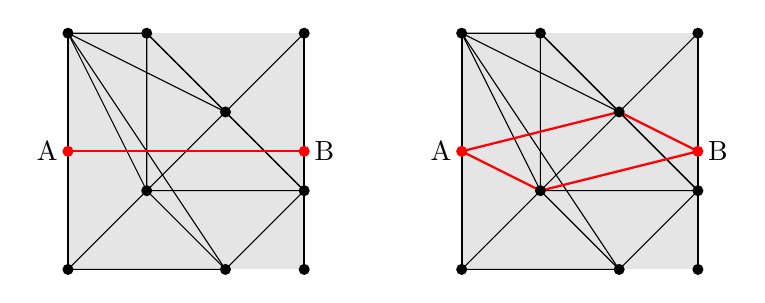
\begin{tikzpicture}
    % Left figure
    \begin{scope}
        % Background
        \fill[gray!20] (0,0) rectangle (3,3);
        
        % Boundary
        \draw[thick] (0,0) -- (0,3);
        \draw[thick] (3,0) -- (3,3);
        
        % Triangulation
        \draw (0,0) -- (1,1) -- (0,3) -- (2,2) -- (3,3) -- (1,1) -- (3,1) -- (2,0) -- (1,1);
        \draw (0,0) -- (2,0) -- (0,3);
        \draw (3,0) -- (3,1) -- (2,2);
        \draw (3,1) -- (1,3) -- (0,3);
        \draw (2,2) -- (1,3) -- (1,1);

        % Line L
        \draw[red, thick] (0,1.5) node[left, black] {A} -- (3,1.5) node[right, black] {B};
        
        % Vertices
        \foreach \x/\y in {0/0, 1/1, 0/3, 2/2, 3/3, 3/0, 2/0, 3/1, 1/3} {
            \fill[black] (\x,\y) circle (2pt);
        }
        
        % Points A and B
        \fill[red] (0,1.5) circle (2pt);
        \fill[red] (3,1.5) circle (2pt);
    \end{scope}
    
    % Right figure
    \begin{scope}[xshift=5cm]
        % Background
        \fill[gray!20] (0,0) rectangle (3,3);
        
        % Boundary
        \draw[thick] (0,0) -- (0,3);
        \draw[thick] (3,0) -- (3,3);
        
        % Triangulation
        \draw (0,0) -- (1,1) -- (0,3) -- (2,2) -- (3,3) -- (1,1) -- (3,1) -- (2,0) -- (1,1);
        \draw (0,0) -- (2,0) -- (0,3);
        \draw (3,0) -- (3,1) -- (2,2);
        \draw (3,1) -- (1,3) -- (0,3);
        \draw (2,2) -- (1,3) -- (1,1);

        % New triangulation from A and B
        \draw[red, thick] (0,1.5) node[left, black] {A} -- (1,1);
        \draw[red, thick] (0,1.5) -- (2,2);
        \draw[red, thick] (3,1.5) node[right, black] {B} -- (1,1);
        \draw[red, thick] (3,1.5) -- (2,2);

        % Vertices
        \foreach \x/\y in {0/0, 1/1, 0/3, 2/2, 3/3, 3/0, 2/0, 3/1, 1/3} {
            \fill[black] (\x,\y) circle (2pt);
        }
        
        % Points A and B
        \fill[red] (0,1.5) circle (2pt);
        \fill[red] (3,1.5) circle (2pt);
    \end{scope}
    
\end{tikzpicture}

\end{document}